\chapter{}{{Methodology}}{Methodology}

Broadly, the proposed framework comprises of the following components:
\begin{enumerate}
    \item Deep feature extraction
    \item Incorporation of auxiliary information
    \item Clustering of auxiliary Information
    \item Multi-label classification of deep features
    \item Predictions of categories/classes
\end{enumerate}

Generally speaking, raw input images carry excess information that is not necessary for the purpose of discrimination and/or fine-grained analysis. Feature extraction enables us to collect important relevant features from an image while discarding the unnecessary information. The deep feature extraction component uses deep neural networks to extract essential information from each image. The first section in this chapter details the feature extraction procedure. Auxiliary information is used by ZSL techniques to learn the relationships between the seen and unseen classes. The second section in this chapter describes the various types of auxiliary information used within the proposed framework. In order to identify representative classes that enable us to predict the large number of unseen classes, we cluster the auxiliary information to find representative cluster centers. The third section in this chapter details the various clustering techniques used. A multi-label classifier is then trained which can discriminate between the representative classes identified in the clustering phase. The fourth section in this chapter describes the classifiers used and their parameters. For a test sample, once the appropriate representative cluster is identified, predictions about unseen classes are made by using a hypothesis generation procedure based on distance measures in the auxiliary space. The fifth section in this chapter describes the distance metrics used to generate the hypotheses from the auxiliary space. Figure \ref{image:overview} depicts a high-level schematic of all the components in the proposed framework.

\begin{sidewaysfigure}
%\begin{figure}[h]

\centering
%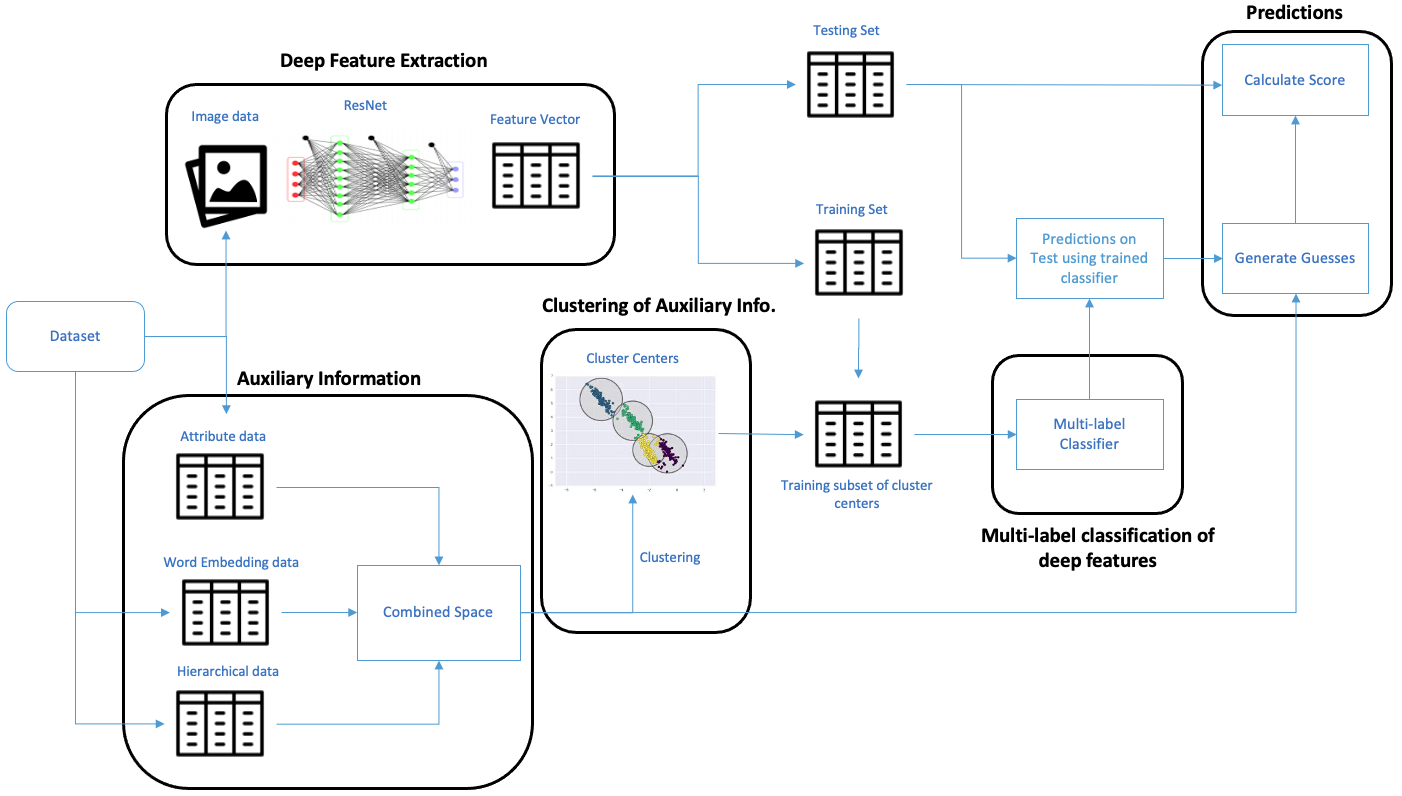
\includegraphics{MS-Thesis-master/figures/overview_new.png}
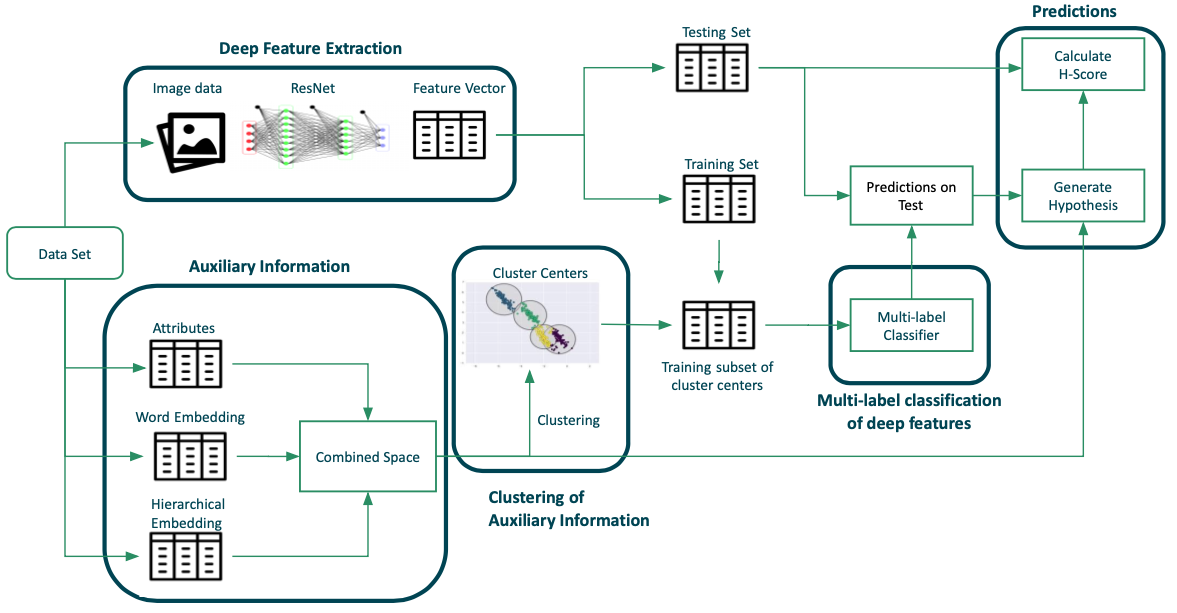
\includegraphics[width=\textwidth]{MS-Thesis-master/figures/overview_latest.png}
%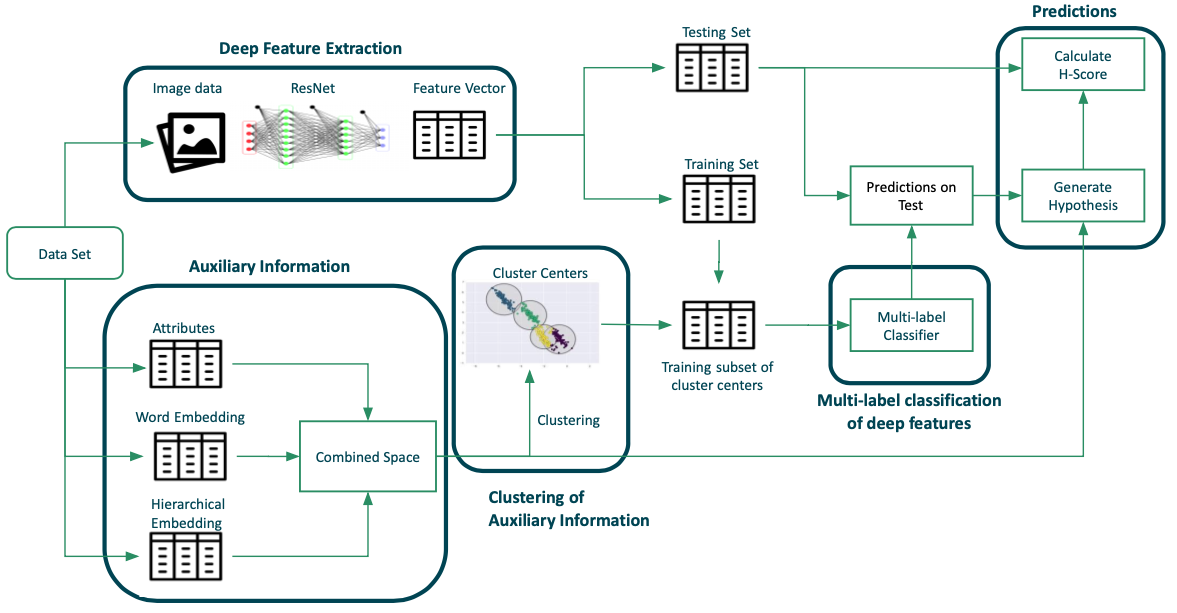
\includegraphics[scale=0.5]{MS-Thesis-master/figures/overview_latest.png}
\caption{High-level schematic of the proposed framework.}
\label{image:overview}
%\end{figure}
\end{sidewaysfigure}

\bigskip
\bigskip

\subchapter{Deep Feature Extraction}

Deep neural networks (DNNs) have proven to perform well for feature extraction from images. We use a ResNet DNN~\cite{resnet} with a depth of 101 layers which is pre-trained on the ImageNet  data set~\cite{imagenet}. This reduces training time significantly and yields useful features since ImageNet consists of over 1 million images spanning 1000 categories. We extract features from the last ResNet layer which translates to 2048 features for each image. ResNet features for all three data sets are also publicly \href{https://www.mpi-inf.mpg.de/departments/computer-vision-and-machine-learning/research/zero-shot-learning/zero-shot-learning-the-good-the-bad-and-the-ugly/}{available}~\cite{gbu}. Figure~\ref{image:resnet_features} shows the architecture and feature extraction map for an image using ResNet-101.

\par
\medskip

Extracted visual features are split into training and testing sets using a stratified 80:20 split. These splits are saved separately for further use in model training and in the prediction phases. Stratified sampling is used so that instances of seen and unseen classes are present in the test set, thus making this a generalized zero-shot learning setting. A seed is used during the splitting phase so that the results can be reproduced. Table \ref{table:train_test_splits} shows a summary of training and testing splits for each data set.

\medskip
\par

\begin{figure}[h!]
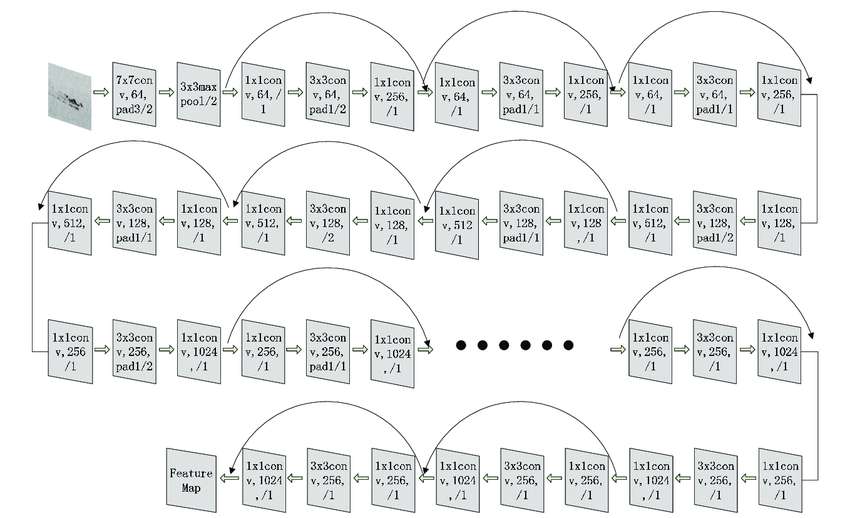
\includegraphics[width=\textwidth]{MS-Thesis-master/figures/ResNet-101-feature-extraction.png}
\caption{ResNet-101 feature extraction map~\cite{resnet-101features}. Each image passes through the network and a feature vector is extracted from the last layer.}
\label{image:resnet_features}
\end{figure}

\par
\medskip

\begin{table}[h!]
\caption{Training and testing splits for each data set}
\centering
\begin{tabular}{@{}lllll@{}}
\toprule
\textbf{Data Set} & \textbf{Classes} & \textbf{Total Images} & \textbf{Training Set Images} & \textbf{Testing Set Images} \\ \midrule
AWA2             & 50               & 37,322          & 29,857                       & 7,465                       \\
CUB              & 200              & 11,788          & 9,430                        & 2,358                       \\
SUN              & 717              & 14,340          & 11,472                       & 2,868                       \\ \bottomrule
\end{tabular}
\label{table:train_test_splits}
\end{table}

\subchapter{Auxiliary Information}

Since instances of unseen classes are unavailable during the training process, auxiliary information is needed to establish semantic relationships between seen and unseen classes, which in turn helps address the ZSL problem. In this framework, we use three sources of auxiliary information for each of the three data sets.

\par
\medskip

\textbf{Attributes.} Humans can naturally perform zero-shot learning with the help of semantic background information. For instance, knowing that "a zebra looks like a horse with stripes" allows us to recognize a zebra without having seen one before, as long as we know what a horse looks like and what the pattern "stripe" looks like \cite{stripes}. All three data sets that are used in this experiment have labelled attribute information for each of their classes. The AWA2 data set~ \cite{awa} includes attributes such as \textit{black}, \textit{small}, \textit{walks}, \textit{smart} etc. with 85 such attributes for each class. The CUB data set ~\cite{cub} includes attributes such as \textit{primary color}, \textit{wing color}, \textit{wing shape}, \textit{size} etc. with 312 such attributes for each class. The SUN data set~\cite{sun} includes attributes such as \textit{man-made}, \textit{natural light}, \textit{medical activity}, \textit{diving} etc. with 102 such attributes for each class.

\par
\medskip

\textbf{Text Embeddings.} A popular idea in modern machine learning is to represent words by vectors that capture hidden information about a language. The learned vector representations for words (i.e., word/text embeddings) from a large general text corpus can help to construct semantic relationships between the seen and unseen class labels. There are three  widely used word embeddings in the research literature: Word2Vec~\cite{w2v}, GloVe~\cite{glove}, and FastText~\cite{fasttext}. FastText has been shown to perform better than the others since it treats each word as composed of character $n$-grams. In FastText the vector for each word is composed as the sum of its character $n$-grams whereas, in Word2Vec and GloVe each word in the corpus is treated as an atomic entity and a unique vector is generated for each word. As a result, FastText can also generate vectors for a combination of words. For instance, "polar bear" has a unique FastText vector representation. FastText has been trained on a very large Wikipedia corpus and is publicly available. In this work, we extract FastText word representations for each class label resulting in a 300-dimensional vector for each class label. 

\par
\medskip

\textbf{Hierarchy Embeddings.} Creating a hierarchy of categories present in a data set allows us to derive taxonomy-based relationships between the classes and improve ZSL performance. For the AWA2 and CUB data sets, Lee et al.~\cite{hnd} propose a two-stage approach for generating hierarchy embeddings where they first derive a top-down hierarchy using WordNet~\cite{wordnet} and then create a flattened hierarchy by representing the probabilities of all the leaf nodes as a single probability vector. Figure~\ref{image:hle} illustrates how hierarchy embeddings are generated for each leaf class in the classification tree. In the case of the AWA2 data set, this results in a 61-dimensional vector and in the case of the CUB data set a 193-dimensional vector. The SUN data set provides its own two-level hierarchy information for each of its 717 categories resulting in a 19-dimensional vector.

\par
\medskip

\begin{figure}[h!]
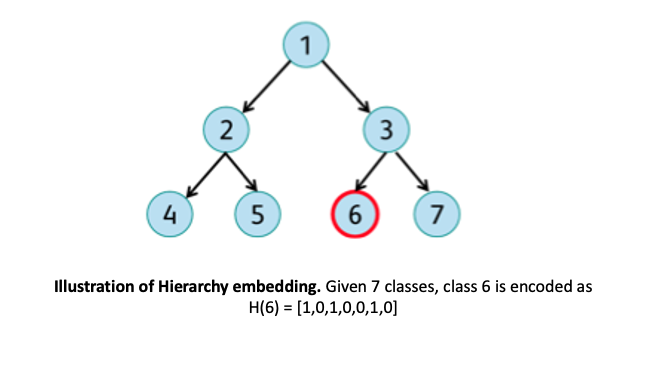
\includegraphics[width=\textwidth]{MS-Thesis-master/figures/hle.png}
\caption{An illustration of hierarchy embedding~\cite{ale}.}
\label{image:hle}
\end{figure}

\textbf{Combined Semantic Space.} The vector spaces of attributes, text embeddings, and hierarchy embeddings are combined into a unified space with reduced dimensions, while retaining the most important information. The dimensionality reduction of the semantic space reduces the computational complexity of the clustering phase and creates robust clusters. We use Principal Component Analysis (PCA) for dimensionality reduction since it retains the variance in the input data while reducing the data dimensionality resulting in a compact combined semantic space. PCA achieves dimensionality reduction by re-projecting the original data along the principal component axes where the principal components are determined via eigenvalue decomposition of the data covariance matrix. The combined, reduced-dimensional semantic space for each data set is computed and retained for use in the clustering and prediction phases. Figures~\ref{image:tsne_awa2}, \ref{image:tsne_cub}, and \ref{image:tsne_sun} show the t-distributed stochastic neighbour embedding (t-SNE) plots~\cite{t-sne} of the combined semantic space for the AWA2, CUB, and SUN data sets respectively. The t-SNE~\cite{t-sne} is a non-linear dimensionality reduction technique that embeds high-dimensional data into a low-dimensional space to aid in data visualization. Specifically, it models each high-dimensional vector as a two- or three-dimensional vector such that similar objects are closer and dissimilar objects are farther apart in the resulting two- or three-dimensional space. In the t-SNE plots for the CUB and SUN data sets, in Figures~\ref{image:tsne_cub} and \ref{image:tsne_sun} respectively, 50 random classes are depicted in the interest of readability. In the t-SNE plots, we observe that classes in the CUB and SUN data set group closer to each other compared to those in the AWA2 data set. This is because AWA2 is a coarse-grained data set whereas CUB and SUN are fine-grained data sets.

\par
\medskip

%\begin{sidewaysfigure}
\begin{figure}[h!]
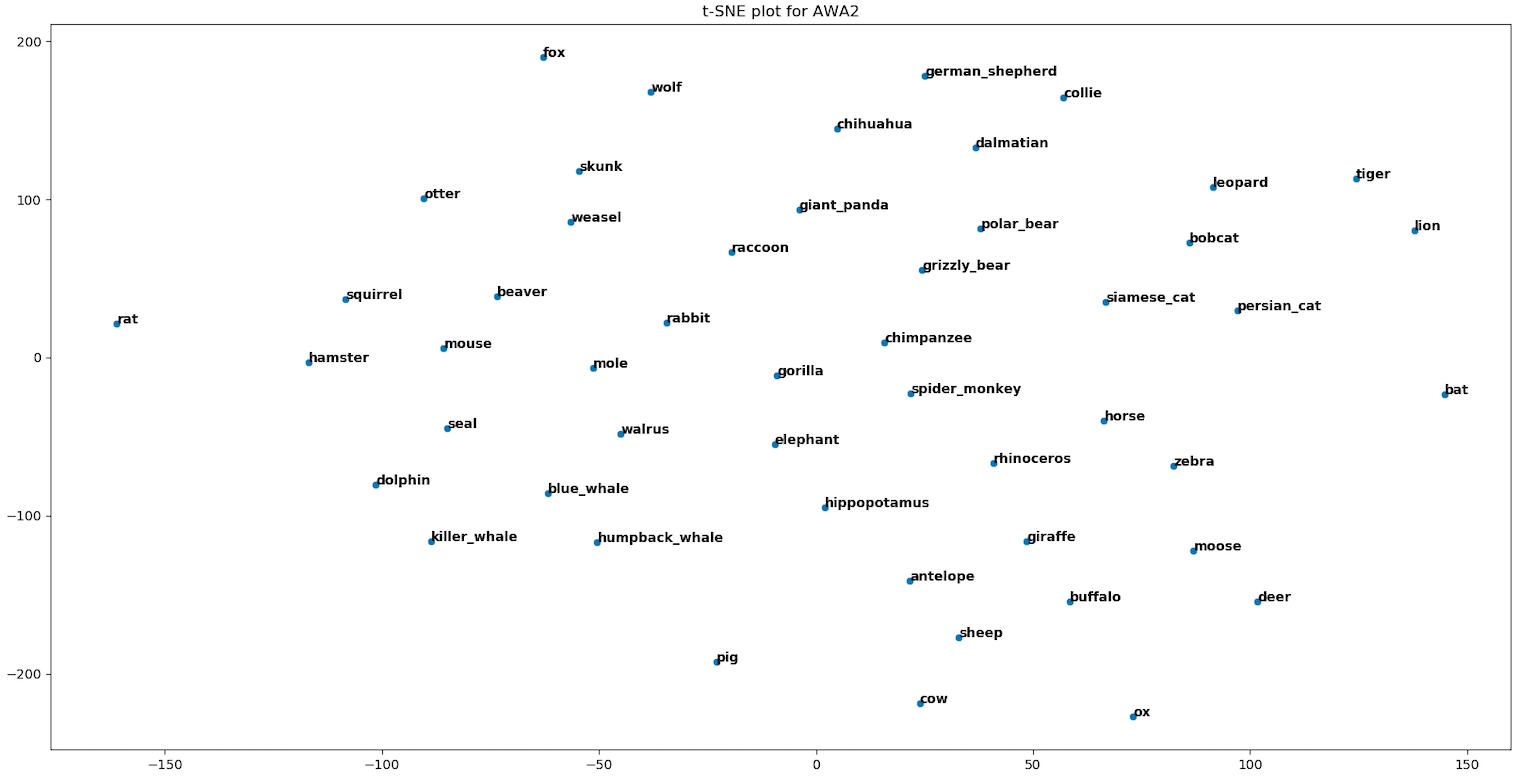
\includegraphics[width=\textwidth]{MS-Thesis-master/figures/tsne_awa2.png}
\caption{t-SNE plot of the combined semantic space in the AWA2 data set with all classes.}
\label{image:tsne_awa2}
\end{figure}

\par
\medskip

%\begin{sidewaysfigure}
\begin{figure}[h!]
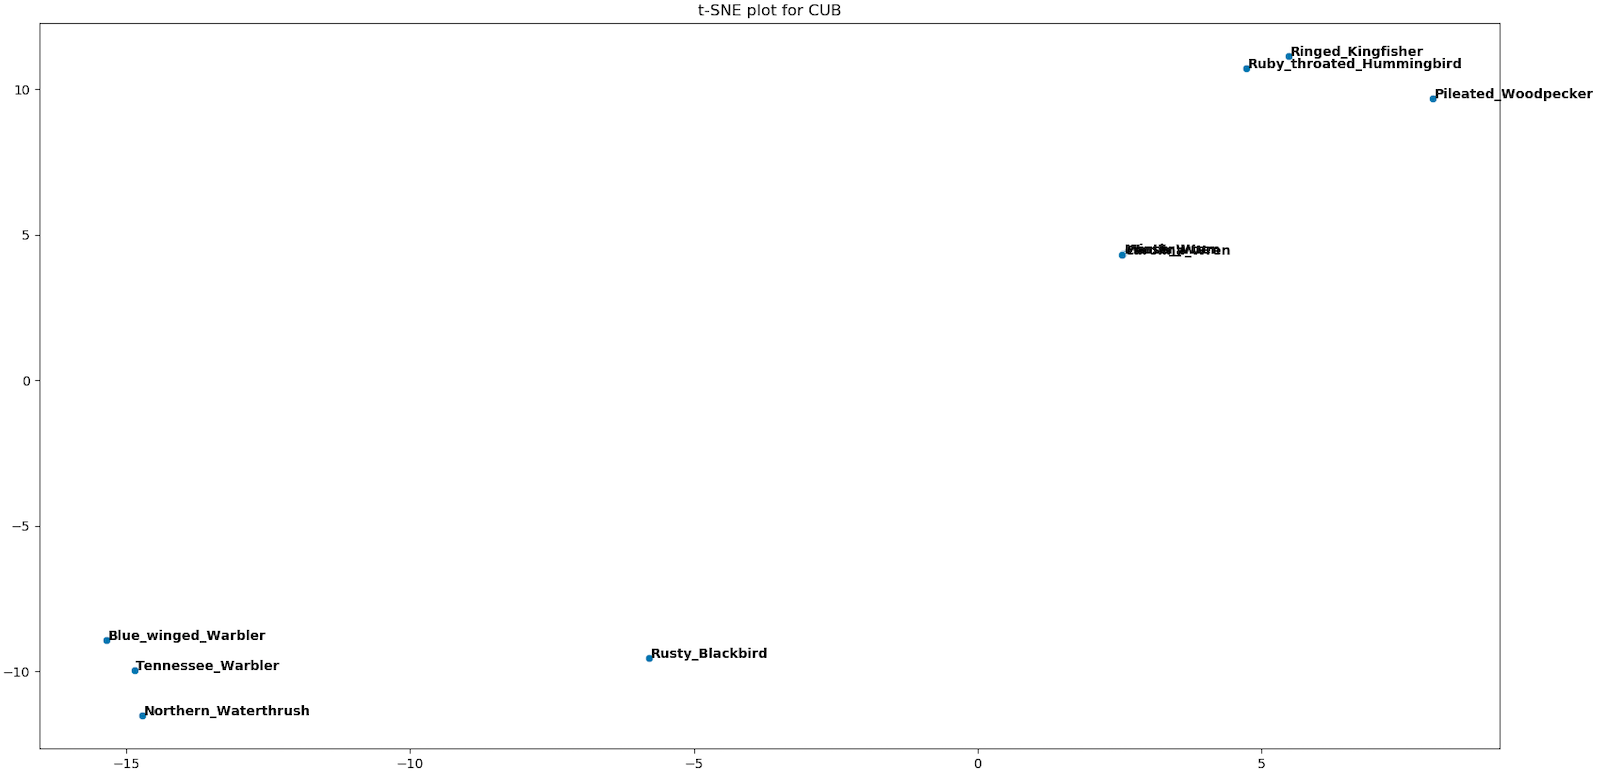
\includegraphics[width=\textwidth]{MS-Thesis-master/figures/tsne_cub_new.png}
\caption{t-SNE plot of the combined semantic space in the CUB data set with 10 classes.}
\label{image:tsne_cub}
\end{figure}

\par
\medskip

\begin{figure}[h!]
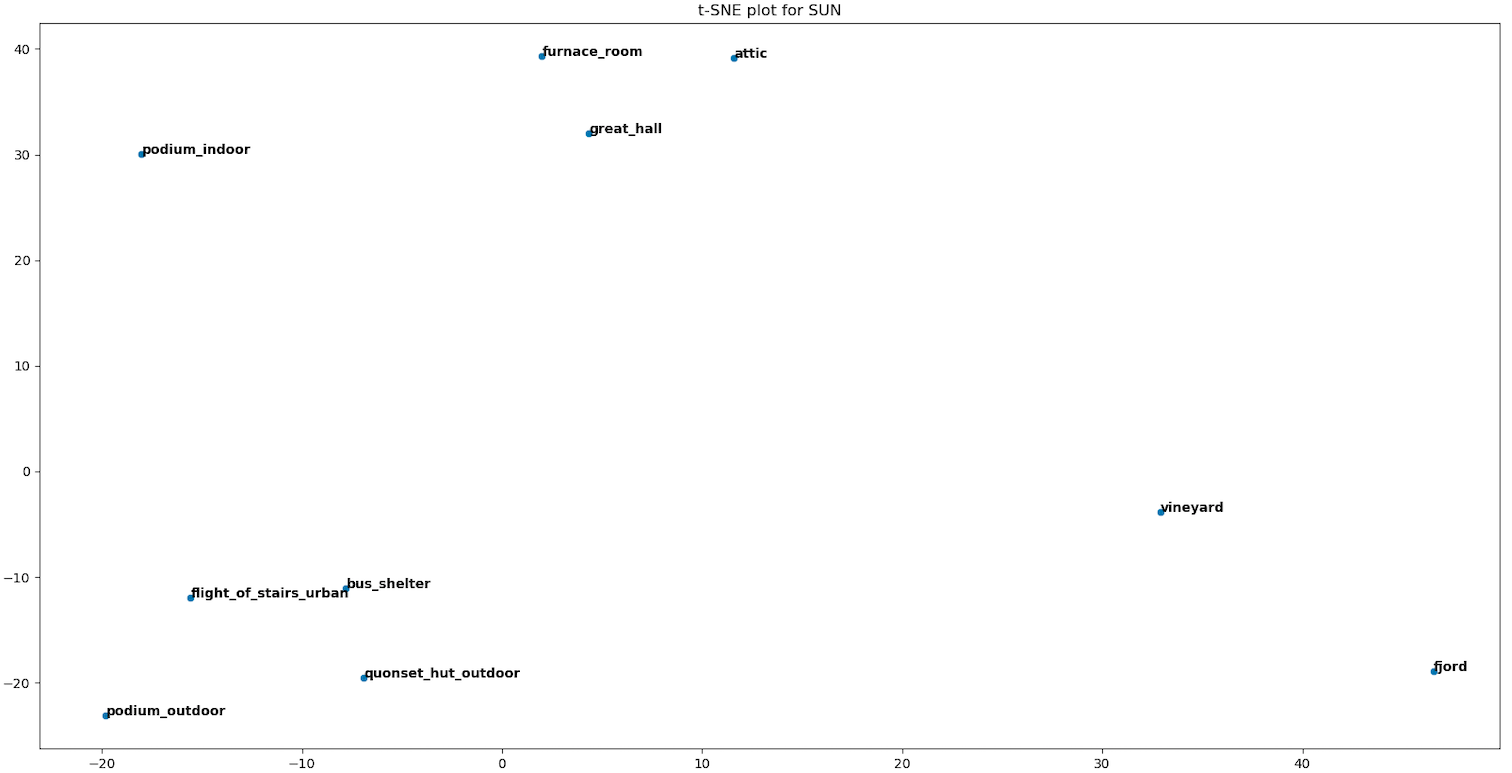
\includegraphics[width=\textwidth]{MS-Thesis-master/figures/tsne_sun_new.png}
\caption{t-SNE plot of the combined semantic space in the SUN data set with 10 classes.}
\label{image:tsne_sun}
\end{figure}

\par
\medskip

\subchapter{Clustering of Auxiliary Information}

The goal of the clustering stage is to identify object categories that are good representatives for a large number of similar object categories. The underlying idea is that these cluster centers would have a strong relationship with its cluster members, thus aiding us to infer cluster members using the cluster centers alone. We use two clustering techniques, i.e., the Gaussian Mixture Model (GMM)~\cite{gmm} and Affinity Propagation (AP)~\cite{affinityprop}, to identify the clusters and representative classes for the clusters. Clustering is performed in the combined reduced-dimensional semantic space for each data set mentioned in the previous section. The clusters centers are noted for further use in the classifier stage.

\par
\medskip

The \textbf{Gaussian Mixture Model (GMM)} can accommodate clusters that have different sizes and correlation structures within them, as opposed to $k$-means clustering. The GMM allows for flexible clustering or soft clustering of the input data. Soft clustering methods assign a score to a data point with respect to each cluster. The value of the score indicates the association strength of the data point to the cluster; in our case the relationship of the data point to the cluster of object categories.  We denote the number of clusters by the variable $k$. GMM-based clustering requires us to specify the number of clusters $k$ before fitting the model. The number of clusters $k$ determines the number of components in the GMM. In our experiments, $k$ starts with a value 5 and ends with a value that equals the total number of classes for a given data set in steps of 5. After identifying all the clusters, the silhouette score~\cite{sil-score} is used to find the optimal value of $k$ for the GMM. 
%%% SMB: ADD THE FOLLOWING CITATION AND REFERENCE FOR silhouette score
%%% P.J. Rousseeuw, Silhouettes: A graphical aid to the interpretation and validation of cluster analysis, Jour. Computational and Applied Mathematics, Vol. 20, 1987, pp. 53-65.

\par
\medskip

\textbf{Affinity Propagation (AP)} is a clustering algorithm based on concept of "message passing" between data points. Unlike the GMM, AP does not require us to specify in advance the number of clusters $k$ to be determined, the algorithm itself provides the optimal number of clusters, i.e., the value of $k$. AP discovers "exemplars" that are members of the input set that are representative of the clusters.

\par
\medskip

The optimal number of clusters for each data set using both clustering techniques is shown in Table \ref{table:k_cl}. It should be noted that since GMM-based clustering was performed using a step size of 5 for $k$, these results may not be the true optimal values for $k$. In this work, we focus primarily on the GMM-based clustering technique since we would like to study how changing number of seen classes i.e. the value of $k$, impacts the classification accuracy.

\par
\medskip

\begin{table}[h!]
\begin{center}
\caption{Optimal number of clusters ($k$ value) for each clustering technique.}
\begin{tabular}{llll}
\hline
\textbf{Data Set} & \textbf{$k$-GMM} & \textbf{$k$-AP} & \textbf{Total Classes} \\ \hline
AWA2 & 15 & 15 & 50\\
CUB & 25 & 24 & 200\\
SUN & 35 & 31 & 717\\ \hline
\end{tabular}
\label{table:k_cl}
\end{center}
\end{table}

\par
\medskip

\subchapter{Multi-label Classification of Deep Features}

After determining the clusters and the representative object for each cluster for different values of $k$, the next step is to train visual classifiers for each cluster center or representative object. A trained visual classifier is used to classify each new test image into one of the representative objects corresponding to the clusters.

\par
\medskip

For each value of $k$, the training set is filtered for the class labels associated with the cluster centers. For example, in the AWA2 data set, for $k = 5$, we have class labels \textit{chimpanzee}, \textit{hamster}, \textit{humpback whale}, \textit{bobcat}, and \textit{ox} as the cluster centers. The image features associated with the class labels of cluster centers alone are considered as the training set and a multi-class visual classifier is trained using this training set. Thus, for each value of $k$, a multi-class classifier is trained, with the training data increasing with increasing number of clusters $k$. Algorithm \ref{algo:cluster_train} shows the steps involved in clustering and training process.

\par
\medskip

\textbf{Visual Classifier.} There are a number of machine learning techniques one can employ to design a multi-class visual classifier such as logistic regression, decision tree, support vector machine (SVM), and neural network. In this work we use a Random Forest (RF) classifier. The RF classifier builds an ensemble of decision trees using a bagging ensemble technique. Simply put, RF builds multiple decision trees and then merges them together to get a more accurate and stable prediction. We use an RF classifier since it is highly scalable for a large number of classes and yields good results. Since we have to train multiple classifiers for varying values of $k$, when using GMM-based clustering, it is difficult to train a neural network or an SVM because of the time complexity and parameter tuning involved. The parameters used in the training of the RF are mentioned in Appendix A.
 
\par
\medskip

\begin{algorithm}[ht]
\SetAlgoLined
\KwData{Combined semantic space, Training set of image features}
\KwResult{Cluster centers and a Trained visual classifier}
 initialization\;
 N $\leftarrow$ Total number of classes in data set\;
 \If{clusteringTechnique = GMM}{
   \For{k in 1 to N with increments of 5}{
  Perform GMM clustering on combined semantic space using k = \textit{k}\;
  Seen classes $\leftarrow$ List of cluster centers\;
  Training subset $\leftarrow$ Subset entire training set for Seen classes alone\;
  Train visual classifier using Training subset\;
  Save classifier
   }
   }
   \If{clusteringTechnique = AF}{
   Perform AF clustering on combined semantic space\;
   Seen classes $\leftarrow$ List of cluster centers\;
   Training subset $\leftarrow$ Subset entire training set for Seen classes alone\;
   Train visual classifier using Training subset\;
   Save classifier
 }
 \caption{Clustering of semantic space and training of visual classifiers. Here, clusteringTechnique denotes the type of clustering technique used. The visual classifier used is a random forest.}
 \label{algo:cluster_train}
\end{algorithm}

\par
\medskip
 
\subchapter{Generation of Predictions or Alternative Hypotheses}
Once visual classifiers are trained, each test instance is classified into one of the representative clusters for a given value of $k$. Alternative hypotheses or predictions are then generated using a similarity measure within the combined semantic space.

\par
\medskip
 
\textbf{Similarity measures.} In machine learning, a similarity measure is an inverse distance metric with dimensionality determined the class feature space. If the distance between two data points is small then there is a high degree of similarity between the classes and vice versa. There are a number of similarity measures using in machine learning such as ones based on Euclidean distance, Manhattan distance, Jaccard distance, and cosine similarity. In this work, we use the cosine similarity measure which computes the cosine of the angle between two vectors as shown in Equation~(\ref{eq:cosine_sim}). Cosine similarity is advantageous because even if the two classes are far apart based on a standard distance metric, it may be possible for their corresponding vectors to be oriented closer together in terms of their angular separation. The smaller the angular separation between the two vectors, the higher the cosine similarity measure.

\par
\medskip
 
\begin{equation}
\label{eq:cosine_sim}
\cos ({\bf a},{\bf b})= {{\bf a} {\bf b} \over \|{\bf a}\| \|{\bf b}\|} = \frac{ \sum_{i=1}^{n}{{\bf a}_i{\bf b}_i} }{ \sqrt{\sum_{i=1}^{n}{({\bf a}_i)^2}} \sqrt{\sum_{i=1}^{n}{({\bf b}_i)^2}} }
\end{equation}

\par
\medskip
 
\textbf{Testing.} Algorithm \ref{algo:test} shows the steps involved in the prediction phase. The test set is split into two subsets. The first subset denotes the seen classes, comprising of data pertaining to class labels that are present in the training set. The second subset denotes the unseen classes, comprising of data pertaining to class labels that are absent from the training set. For each of these subsets, we determine top prediction using the trained visual classifier and then find the closest class label in the combined semantic space using the cosine similarity measure. Classification accuracy is computed for each subset separately followed by the computation of the \textit{harmonic score} (H-score) using Equation~(\ref{eq:hscore}).

\par
\medskip
 
\begin{equation} 
\label{eq:hscore}
\ H-score= \frac{2 *(Seen Class Accuracy)*(Unseen Class Accuracy)}{(Seen Class Accuracy)+(Unseen Class Accuracy)}\
\end{equation}

\par
\medskip
 
We choose the harmonic mean as the performance metric instead of the arithmetic mean because in the case of the latter, if the seen class accuracy is much higher than the unseen class accuracy, the overall arithmetic mean is significantly skewed towards the seen class accuracy~\cite{gbu}. However, since our aim is to attain high classification accuracy on both the seen and unseen classes, the harmonic mean is a better quantifier of overall classification accuracy.

\par
\medskip
 
\begin{algorithm}[ht]
\SetAlgoLined
\KwData{Combined semantic space, Trained Classifiers, Trained Clusters, Testing set of image features}
\KwResult{Overall H-Score on the test set}
 initialization\;
 N $\leftarrow$ Total number of classes in data set\;
 C $\leftarrow$ List of all class labels in data set\;
 \If{clusteringTechnique = GMM}{
   \For{k in 1 to N with increments of 5}{
  Cluster centers $\leftarrow$ List of cluster centers from clusters trained using k = \textit{k}\;
  Seen classes $\leftarrow$ Subset test set for Cluster centers alone\;
  Unseen classes $\leftarrow$ Subset test set for  [C - Cluster centers]\;
  Use classifier trained for k=\textit{k} to predict on seen and unseen classes\;
  Use cosine similarity to find closest neighbour in Combined semantic space\;
  Calculate accuracy\;
  Calculate H-Score\;
   }
   }
   \If{clusteringTechnique = AF}{
  Cluster centers $\leftarrow$ List of cluster centers from clusters trained using k = \textit{k}\;
  Seen classes $\leftarrow$ Subset test set for Cluster centers alone\;
  Unseen classes $\leftarrow$ Subset test set for  [C - Cluster centers]\;
  Use classifier trained for k=\textit{k} to predict on seen and unseen classes\;
  Use cosine similarity to find closest neighbour in Combined semantic space\;
  Calculate accuracy\;
  Calculate H-Score\;
 }
 \caption{Prediction phase algorithm. Here, clusteringTechnique denotes the type of clustering technique used.}
 \label{algo:test}
\end{algorithm}

\newpage